\documentclass[12pt,a4paper]{article}

% --- Paketler ---
\usepackage[utf8]{inputenc}
\usepackage[T1]{fontenc}
\usepackage[turkish]{babel} % Türkçe dil desteği
\usepackage{amsmath} % Matematiksel formüller
\usepackage{geometry} % Sayfa kenar boşlukları
\geometry{a4paper, margin=2.5cm}
\usepackage{hyperref} % Tıklanabilir linkler
\usepackage{graphicx} % Resim eklemek için
\usepackage{titlesec} % Başlık formatlaması
\usepackage{setspace} % Satır aralığı (1.5)
\onehalfspacing
\usepackage{tikz} % Kodla çizim için (Graph)
\usepackage{pgfplots} % Kodla çizim için (Graph)
\usetikzlibrary{shapes.geometric, arrows.meta, babel} % babel kütüphanesi çakışmaları önler
\pgfplotsset{compat=1.18}
\usepackage{xcolor} % Uyarı metni için

% --- Doküman Bilgileri ---
\title{\textbf{TUA AYAP-2 Otonom Gezen Araç}\\ \Large Hiyerarşik ve Çok Amaçlı Dinamik Rota Optimizasyonu Mimarisi}
\author{Eren Köse\\ \normalsize Türkiye Uzay Ajansı (TUA) / TUA Hackathon}
\date{28 Mart 2026}

\begin{document}
% DİKKAT: Turkish babel paketinin "=" ve ":" işaretlerini bozarak Graphicx ve TikZ'i 
% sonsuz döngüye sokmasını (Compile Timeout) engellemek için aşağıdaki komut şarttır:
\shorthandoff{=}

\maketitle

% --- Özet ---
\begin{abstract}
Bu rapor, Türkiye Uzay Ajansı (TUA) Ay Araştırma Programı-2 (AYAP-2) hedefleri doğrultusunda, Ay yüzeyinde görev yapacak otonom bir gezen araç için geliştirilmiş Hiyerarşik ve Çok Amaçlı Dinamik Rota Optimizasyonu mimarisini sunmaktadır. Sistem, kısıtlı uzay donanımları üzerinde (RAD750 vb.) devasa Ay topoğrafya verilerini işleyebilmek için Hiyerarşik Kayar Pencere (Sliding Window) mimarisini kullanır. Rota seçimi, sadece mesafeyi değil; eğim (devrilme riski), terramekanik (patinaj/sinkage) ve güneş ışınımı (termal/enerji ödülü) metriklerini harmanlayan 4 Boyutlu bir maliyet fonksiyonu ile dinamik olarak optimize edilir. Geliştirilen mimari, aracın kilitlenmesini önleyerek hayatta kalma ihtimalini en üst düzeye çıkarmayı hedeflemektedir.
\end{abstract}

\newpage

% --- Giriş ve Ana Hedef ---
\section{Giriş ve Ana Hedef}
Bu proje, Türkiye Uzay Ajansı (TUA) Ay Araştırma Programı-2 (AYAP-2) hedefleri doğrultusunda, Ay yüzeyinde görev yapacak otonom bir gezen araç (rover) için geliştirilmiş Hiyerarşik ve Çok Amaçlı Dinamik Rota Optimizasyonu mimarisidir. 24 saat içerisinde sağlanan küresel uydu verileriyle (1 metrelik Haworth Krateri DEM) Ay yüzeyi üzerinde "Google Maps" benzeri bir otonom haritalama sistemi kurmak temel amacımızdır.

Bu harita üzerinde otonom aracın sadece en kısa değil, uzay şartlarında "hayatta kalma ihtimali en yüksek (en optimum)" yolu bulmasını; uzay aviyoniklerinin (RAD750 vb.) dar RAM ve CPU kapasitelerini kilitlenmekten kurtaran Hiyerarşik Kayar Pencere (Sliding Window) mimarisi ve 4 temel metriğe dayanan Çok Amaçlı Modifiye A* algoritması ile sağlamaktayız.
\section{Ay Yüzeyinin Fiziksel Karakteristiği ve Algoritmik Tasarıma Etkisi}
Otonom bir gezen aracın (rover) Dünya üzerindeki navigasyonu ile Ay üzerindeki navigasyonu arasında devasa uçurumlar bulunmaktadır. Bu projenin temelini oluşturan Hiyerarşik ve Çok Amaçlı Dinamik Rota Optimizasyonu mimarisi, salt matematiksel bir yol bulma problemi olarak değil; Ay'ın, özellikle de Güney Kutbu'nun acımasız fiziksel gerçekliklerine karşı bir "hayatta kalma mekanizması" olarak tasarlanmıştır.

Ay'ın çevresel faktörleri ve bu faktörlerin projemizdeki doğrudan karşılıkları aşağıda detaylandırılmıştır:

\subsection{Güney Kutbu, Aydınlatma Dinamikleri ve Termal Uçurumlar}
\textbf{Ay'ın Gerçekliği:} TUA AYAP-2 hedefleri doğrultusunda aracın inmesi planlanan Ay'ın Güney Kutbu (Haworth Krateri bölgesi), Güneş ışınlarını neredeyse tamamen yatay bir açıyla alır. Bu durum, krater içlerinde sıcaklığın $-200^\circ\text{C}$'nin altına düştüğü Kalıcı Gölge Bölgeleri (Permanently Shadowed Regions - PSR) yaratır. Atmosfer olmadığı için aydınlık bir tepe ile karanlık bir krater tabanı arasındaki termal uçurum, aracın batarya ve elektronik sistemlerini anında dondurma riskine sahiptir.

\textbf{Algoritmamıza Yansıması:} Bu ölümcül termal gerçeklik, maliyet fonksiyonumuzdaki \textbf{Gölge ($G$)} parametresinin doğmasını sağlamıştır. Sistemimiz, basit bir harita navigasyonunun ötesine geçerek ışın izleme (ray casting) verisini kullanır. Araç, donmamak ve güneş panellerini aktif tutmak için gölgelerden "esnek kaçınma" stratejisi güder ve SoC (Batarya) seviyesi düştüğünde hayatta kalma içgüdüsüyle Güneş alan zirvelere yönelir.

\subsection{Regolit Zemin ve Düşük Yerçekimi ($1/6\,G$)}
\textbf{Ay'ın Gerçekliği:} Ay'da Dünya'nın sadece altıda biri ($1/6$) oranında yerçekimi bulunur. Ayrıca yüzey, milyarlarca yıllık meteorit çarpmaları sonucu un ufak olmuş, pudra şekeri kıvamındaki "regolit" adı verilen ince ay tozu ile kaplıdır. Düşük yerçekimi aracın yere tutunma kuvvetini (traksiyon) dramatik ölçüde azaltırken, regolit zemin tekerleklerin kuma gömülmesine (sinkage) veya boşa dönmesine (slip/patinaj) neden olur.

\textbf{Algoritmamıza Yansıması:} Klasik algoritmalar zemini düz bir düzlem olarak varsayar. Bizim mimarimizde ise bu gerçeklik \textbf{Sürtünme ($S$)} ve \textbf{Eğim ($E$)} parametreleri ile formüle edilmiştir. Algoritma, patinaj ve batma riski yüksek regolit havuzlarını tespit ederek bu bölgelere yüksek ceza keser. Ayrıca düşük yerçekiminde aracın devrilme riski çok daha yüksek olduğu için, eğim maliyeti "Asimetrik U-Eğrisi" mantığıyla çalışarak dik yokuş çık
% --- RESİM: GÖREV KONSEPTİ VE AY YÜZEYİ ---
\begin{figure}[h]
    \centering
    % Görseller sisteme yüklenene kadar hata vermemesi için \rule (boş kutu) eklendi.
    % Resimleri yüklediğinizde \rule satırını silip \includegraphics satırının başındaki % işaretini kaldırın.
    \rule{\textwidth}{6cm}
    % \includegraphics[width=1.0\textwidth]{resimler/ay_guney_kutbu_konsept.png}
    \caption{TUA AYAP-2 Otonom Gezen Araç Misyon Konsepti. Görsel, Ay Güney Kutbu’ndaki zorlu topoğrafyayı ve kalıcı gölge bölgelerini kavramsal olarak göstermektedir.}
    \label{fig:gorev_konsepti}
\end{figure}

% --- Maliyet Fonksiyonu ---
\section{Dört Boyutlu (4D) Çok Amaçlı Maliyet Fonksiyonu ve Optimizasyon Detayları}
Standart navigasyonlar sadece "en kısa mesafeyi" en iyi yol sanır. Bizim sistemimizin beyni ise, Ay’ın fiziksel gerçekliklerini yansıtan 4 temel metriği harmanlayarak karar verir. Bu metriklerin birbirlerine olan ağırlıkları ve matematiksel limitleri, projeye özel geliştirilecek istatistiksel bir formülle dinamik olarak belirlenmektedir.

Navigasyon sistemimizin karar mekanizması, bu 4 temel metriğin matematiksel bir sentezidir. Toplam maliyeti ($C_{toplam}$) hesaplayan temel denklem şu şekildedir:

\begin{equation}
C_{toplam} = \left[ (W_d \cdot D) + (W_e \cdot E) + (W_s \cdot S) - (W_g \cdot G) \right] \times 1000
\end{equation}

\textit{Buradaki $W$ değerleri, aracın batarya durumuna göre değişen dinamik ağırlıkları temsil eder. Tam şarj durumunda temel ağırlıklar: $D = \%30$, $E = \%45$, $S = \%15$, $G = \%10$ olarak belirlenmiştir.}

\subsection{Mesafe (D): Kinematik Enerji ve İlerleme Puanı}
Klasik navigasyonlarda mesafe sadece bir uzunluk birimidir. Bizim modelimizde ise mesafe, aracın "baz enerji tüketimi" (baseline power draw) anlamına gelir. Bu metrik, aracın haritada gereksiz yere gezinmesini engelleyen ve onu sürekli nihai hedefe doğru çeken "mıknatıs" görevi görür. Araç, hayatta kalma kısıtları elverdiği sürece en kısa rotayı bulmaya çalışır.

\subsection{Eğim (E): Asimetrik U-Eğrisi ve Devrilme Riski}
Ay’daki düşük yerçekimi (1/6 G) nedeniyle aracın yere tutunma kuvveti çok zayıftır. Algoritmamız, matematiksel çökmeleri (sonsuz döngü) engellemek için negatif maliyet kullanmak yerine, NASA’nın gezegen keşif araçlarında uyguladığı "Asimetrik U-Eğrisi" maliyet mantığını kullanır:
\begin{itemize}
    \item \textbf{Düz Yollar:} Standart maliyettedir.
    \item \textbf{Hafif İnişler:} Motoru yormadığı ve rejeneratif frenleme sağladığı için algoritmada "sıfıra en yakın (minimum)" maliyetle bir ödül olarak işlenir; böylece araç güvenli vadilerden süzülmeye teşvik edilir.
    \item \textbf{Dik Çıkışlar:} Bataryayı sömürdüğü için üstel (exponential) olarak artan yüksek cezalar alır.
\end{itemize}

% --- RESİM: ASİMETRİK U-EĞRİSİ MANTIĞI (TikZ ile) ---
\begin{figure}[h]
    \centering
    \begin{tikzpicture}
        \begin{axis}[
            width=12cm, height=7cm,
            axis lines=middle,
            xlabel={\textbf{Eğim} (Yokuş Aşağı $\leftarrow$ 0 $\rightarrow$ Yokuş Yukarı)},
            ylabel={\textbf{Maliyet} ($C_e$)},
            xmin=-5, xmax=5,
            ymin=0, ymax=10,
            xtick=\empty, ytick=\empty,
            domain=-4:4,
            samples=40, 
            thick,
            every axis x label/.style={at={(ticklabel* cs:1.05)}, anchor=west,},
            every axis y label/.style={at={(ticklabel* cs:1.05)}, anchor=south,}
        ]
        
        % Asimetrik U-Eğrisi Formülü (Kavramsal Temsil)
        \addplot [blue, ultra thick] {exp(0.6*x) + 0.15*x^2 + 1};
        
        % Etiketler
        \node[label={270:{\small Rejeneratif Ödül}}] at (axis cs:-2.5, 2.5) {};
        \node[label={180:{\small Üstel Ceza (Devrilme Riski)}}] at (axis cs:3, 8) {};
        
        % Çizgilerle bölge gösterme
        \draw[dashed, red] (axis cs:0,0) -- (axis cs:0,10);
        
        \end{axis}
    \end{tikzpicture}
    \caption{Eğim Maliyeti ($C_e$) Fonksiyon Grafiği. Araç, güvenli inişleri (regenerative braking) ödüllendirirken, dik çıkışlara karşı hayatta kalma içgüdüsüyle üstel bir ceza keser.}
    \label{fig:asimetrik_egri}
\end{figure}

\subsection{Sürtünme ve Terramekanik (S): Batma ve Patinaj Riski}
Eğim sıfır olsa bile Ay yüzeyi homojen değildir; bazı yerler sert kaya, bazı yerler ise pudra şekeri kıvamında gevşek regolittir (ay kumu). Gevşek zeminde tekerlek boşa döner (patinaj/slip). Araç ilerleyemediği halde motorlar tam güç çalıştığı için batarya sömürülür ve en kötüsü tekerlek kuma gömülerek (sinkage) araç tamamen kilitlenir. Bu metrik, zeminin pürüzlülük ve sertlik durumunu değerlendirerek patinaj ve kuma gömülme riski yüksek, sürtünmesi zayıf bölgelere yüksek ceza faturası keser ve aracı daha sağlam rotalara yönlendirir.

\subsection{Gölge (G): Termal Tolerans ve Esnek Gölge İzolasyonu}
Ay’ın Güney Kutbu’nda güneş ışınları yatay açıyla gelir ve eksi 200 dereceleri bulan karanlık krater gölgeleri yaratır. Otonom araçlarda aracı sürekli güneşe yönlendiren "ödül" sistemleri, aracın hedefi unutup panellerini güneşte tutmak için kendi etrafında dönmesine (Günebakan Etkisi) yol açar. Bu yüzden sistemimiz, "esnek (soft) kaçınma" mantığıyla çalışır. Pikselin aydınlık durumu Işın İzleme (Ray Casting) teknolojisiyle tespit edilir.
\begin{itemize}
    \item \textbf{Aydınlık Pikseller:} $G = 1$ (Güvenli)
    \item \textbf{Karanlık Pikseller:} $G = 50$ (Yüksek Maliyet)
\end{itemize}
Karanlık pikseller aşılmaz birer duvar (sonsuz ceza) değildir; yüksek geçiş maliyeti üreten bölgelerdir. Eğer karanlık bir kraterin içinden geçmek, araca ciddi bir mesafe (D) ve güvenli bir eğim (E) avantajı sağlıyorsa, algoritma bu "hesaplanmış termal riski" göze alıp gölgeden ilerleyebilir. Aksi takdirde araç sadece aydınlık zirvelere hapsolur ve operasyonel hareket kabiliyetini yitirir.

\newpage

% --- Dinamik Şarj ---
\section{Dinamik Şarj (SoC) Adaptasyonu ve Hayatta Kalma İçgüdüsü}
Modelimizi diğer tüm algoritmalardan ayıran özellik, aracın kendi "açlık" durumunu fark edebilmesidir. Formüldeki Gölge Ağırlığı ($W_g$), aracın Batarya Şarj Durumuna (SoC) bağlı olarak çalışan bir parçalı fonksiyon (piecewise function) ile sürekli güncellenir. Batarya seviyesi ($B$) üzerinden tepki senaryosu şu şekildedir:
\begin{itemize}
    \item \textbf{$B > \%50$ (Güvenli):} $W_g = 0.10$ | Araç ufak gölgeleri umursamaz, hedefe odaklanır.
    \item \textbf{$\%20 < B \le \%50$ (Uyarı):} $W_g = 0.40$ | Gölgelerden kaçınma eğilimi ciddi şekilde artar.
    \item \textbf{$B \le \%20$ (Kritik - Hayatta Kalma Modu):} $W_g = 0.80$ | Formülün bütün gücü gölge maliyetine aktarılır ($0.80 \times 50 = 40$ ceza puanı). Maliyetler devasa seviyelere fırladığı için araç hedefine gitmeyi iptal eder ve donmamak için anında en yakın aydınlık tepeye (Safe Haven) rotasını çevirir.
\end{itemize}

% --- Maliyet Detayları ---
\section{Maliyet Fonksiyonu Parametrelerinin Davranışsal Analizi}
Otonom aracın karar mekanizmasını oluşturan 4 temel metrik, toplam maliyet skorunu ($C_{toplam}$) farklı yönlerde ve şiddetlerde etkiler. Her bir parametrenin sisteme matematiksel etkisi ve fiziksel yorumu aşağıda detaylandırılmıştır:

\subsection{Mesafe (D) $\rightarrow$ Maliyeti ARTTIRIR}
\textbf{Karakteristik:} Mesafe uzadıkça motorların aktif kalma süresi artar ve bu durum toplam maliyeti standart bir oranda yukarı çeker. \\
\textbf{Fiziksel Yorum:} Mesafe tek başına belirleyici bir parametre değildir. Diğer hayati risklerin (eğim, gölge, patinaj) eşit olduğu durumlarda, alternatif rotaları birbirinden ayırmak için bir eşitlik bozucu (tie-breaker) olarak görev yapar. Aracın haritada gereksiz dolaşmasını engeller.

\subsection{Eğim (E) $\rightarrow$ Maliyeti ŞİDDETLE ARTTIRIR}
\textbf{Karakteristik:} Formüldeki katsayısı (0.45) en yüksek parametredir. Eğim arttıkça maliyet skoru üstel olarak fırlar. \\
\textbf{Fiziksel Yorum:} Gezginin yerçekimine karşı iş yapması, bataryayı en hızlı tüketen ve mekanik stresi en çok artıran faktördür. Aracın devrilme açısı (tip-over angle) sınırına yaklaşılması kritik bir risktir. Bu nedenle, hesaplanan eğim kritik devrilme sınırını aşarsa, bu değer normalize formüle girmeden önce algoritmada bir if koşulu ile yakalanır. Bu durumda maliyete direkt olarak $\infty$ (veya pratik bir maksimum ceza değeri, örn. 10000) atanarak o yol tamamen iptal edilir.

\subsection{Sürtünme ve Terramekanik (S) $\rightarrow$ Maliyeti ARTTIRIR}
\textbf{Karakteristik:} Zemin bozuldukça ve pürüzlülük arttıkça $S$ değeri 1’e yaklaşır ve maliyeti belirgin ölçüde yukarı çeker. \\
\textbf{Fiziksel Yorum:} Gidilecek zemin kayalık, yumuşak kum (regolit) veya çamur yapısında ise tekerleklerin "slip" (patinaj/kayma) oranı artar. Aracı ilerletmek için tekerleklere daha fazla tork verilmesi gerekir. Bu durum hem enerji tüketimini artırır hem de kuma gömülme (sinkage) riski doğurur.

\subsection{Güneşin Konumu (G) $\rightarrow$ Maliyeti AZALTIR}
\textbf{Karakteristik:} Maliyet fonksiyonundaki tek negatif ($-$) çarpanlı faktördür. Rota güneşe dönükse maliyet skorunu aşağı çekerek (iyileştirerek) o rotayı cazip hale getirir. \\
\textbf{Fiziksel Yorum:} Araç, güneşli bir rotada ilerlerken panelleri verimli ışınım alır ve bataryayı eşzamanlı olarak şarj eder. Harcanan net enerji düşeceği için sistem, bu durumu bir "ödül" olarak işler. Bu sayede otonom araç, kısa ama karanlık bir krater yolu yerine; biraz daha uzun ama bol güneş alan, enerji verimliliği yüksek rotaları tercih etme eğilimi gösterir.

\newpage
\section{Navigasyonun Kalbi: Modifiye Çok Amaçlı A* Algoritması}
Geliştirilen otonom navigasyon sisteminin temel karar motoru, klasik yol bulma algoritmalarının uzay şartlarına uyarlanmış bir versiyonu olan \textbf{Modifiye Çok Amaçlı A* (A-Star)} algoritmasıdır.

\subsection{Standart A* Algoritmasının Teorik Altyapısı}
A* algoritması, bilgisayar bilimlerinde bilinen en verimli ve yaygın sezgisel (heuristic) yol bulma algoritmalarından biridir. Algoritma, her bir düğümün (node/piksel) maliyetini aşağıdaki temel fonksiyon ile hesaplar:
\begin{equation}
f(n) = g(n) + h(n)
\end{equation}
\begin{itemize}
    \item \textbf{$f(n)$:} Başlangıç noktasından hedefe, $n$ düğümü üzerinden geçen yolun tahmini toplam maliyeti.
    \item \textbf{$g(n)$:} Başlangıç noktasından mevcut $n$ düğümüne kadar gelmek için harcanan kesinleşmiş maliyet.
    \item \textbf{$h(n)$:} Mevcut $n$ düğümünden nihai hedefe ulaşmak için kalan tahmini sezgisel maliyet (Heuristic). Genellikle Öklid (Euclidean) veya Manhattan mesafesi kullanılır.
\end{itemize}

\subsection{AYAP-2 Mimarisinde A* Algoritmasının Konumu ve Rolü}
Standart navigasyon sistemlerinde A* algoritması tüm haritayı baştan sona tarayarak tek bir seferde çalışır. Ancak 1 metre çözünürlüklü devasa Haworth Krateri verisi üzerinde bu yaklaşım RAD750 gibi dar kapasiteli aviyonikleri anında kilitler.

Bu projede A* algoritması, tüm haritada koşturulmak yerine \textbf{Hiyerarşik Kayar Pencere (Sliding Window)} mimarisinin lokal (mikro) işlem katmanında çalıştırılır. 
\begin{itemize}
    \item Global katman, devasa harita üzerinden düşük çözünürlüklü bir "kılavuz çizgi" çizer ve araca belirli aralıklarla "alt hedefler" (sub-goals) verir.
    \item Aracın işlemcisi, sadece etrafındaki $100 \times 100$ piksellik aktif Kayar Pencere içerisindeki yüksek çözünürlüklü veriyi RAM'e alır. 
    \item \textbf{A* Algoritması tam bu aşamada devreye girer:} Sadece bu dar pencere sınırları içerisinde, aracın bulunduğu noktadan bir sonraki alt hedefe giden en güvenli mikro rotayı adım adım hesaplar. Pencere araçla birlikte kaydıkça, A* algoritması da sürekli olarak kendini yenileyen bu lokal alan üzerinde yeniden koşturulur.
\end{itemize}

\subsection{Standart A*'dan "Modifiye Çok Amaçlı" A*'a Geçiş}
Standart A* algoritmasında $g(n)$ değeri genellikle sadece "kat edilen fiziksel mesafedir". Ancak Ay yüzeyinde en kısa yol, genellikle en ölümcül yoldur. Algoritmamızı literatürdeki klasik A* kullanımlarından ayıran en temel yenilik, $g(n)$ maliyet fonksiyonunun tamamen değiştirilmesidir.

Modelimizde A* algoritmasının $g(n)$ hesaplaması, basit bir uzunluk ölçümü olmak yerine daha önce denklem (1)'de tanımladığımız \textbf{4 Boyutlu Maliyet Fonksiyonuna ($C_{toplam}$)} eşitlenmiştir:
\begin{equation}
g(n) = C_{toplam} = \left[ (W_d \cdot D) + (W_e \cdot E) + (W_s \cdot S) - (W_g \cdot G) \right] \times 1000
\end{equation}

Bu modifikasyon sayesinde algoritmamız sıradaki piksele gitmeyi değerlendirirken; 
1) Sadece mesafeye bakmaz, o pikselin eğiminden doğacak devrilme riskini ($E$) hesaba katar.
2) Zeminin regolit (kum) yapısına bakarak patinaj ve batma riskini ($S$) değerlendirir.
3) O pikselin güneş mi yoksa derin gölge mi olduğuna ($G$) bakarak termal toleransı hesaplar.

Sonuç olarak sezgisel $h(n)$ fonksiyonu aracı ısrarla hedefe doğru bir mıknatıs gibi çekerken; çok amaçlı $g(n)$ fonksiyonumuz, bu çekim kuvvetine karşı koyarak aracın dik yamaçlardan, gevşek kumlardan ve donma tehlikesi olan derin krater gölgelerinden kaçınmasını (hayatta kalmasını) sağlar.
\section{A* (A-Yıldız) Algoritmasının Teorik Temelleri ve Karakteristiği}
Geliştirilen otonom navigasyon sisteminin kalbinde yatan karar motorunu tam olarak kavrayabilmek için, öncelikle işin alfabesi olan klasik A* (A-Star) algoritmasının doğasını ve çalışma mekaniğini incelemek gerekmektedir. A*, bilgisayar bilimlerinde, robotikte ve yapay zeka alanında A noktasından B noktasına gitmek için kullanılan en verimli ve yaygın yol bulma (pathfinding) algoritmasıdır.

\subsection{A* Algoritması Nedir?}
A* algoritmasının literatürdeki eşsiz konumu, iki farklı klasik algoritmanın en güçlü yönlerini birleştirmesinden kaynaklanır:
\begin{itemize}
    \item \textbf{Dijkstra Algoritması:} Hedefe giden en kısa yolu bulmayı kesin olarak garanti eder, ancak "hedefin nerede olduğunu" bilmediği için haritadaki her yöne körlemesine yayılarak çalışır (hesaplama maliyeti çok yüksektir).
    \item \textbf{Açgözlü En İyi Öncelikli Arama (Greedy Best-First Search):} Sadece hedefe doğru yönelir ve çok hızlıdır; ancak karşısına bir engel (duvar, krater) çıktığında optimal (en kısa) yolu bulmayı garanti edemez.
\end{itemize}
A* algoritması, Dijkstra'nın \textit{kesinliğini} ve Açgözlü aramanın \textit{hedefe kilitlenme (sezgisel)} yeteneğini harmanlar. Hem en kısa yolu bulmayı garanti eder hem de bunu gereksiz alanları taramadan, doğrudan hedefe yönelerek yapar.

\subsection{Matematiksel Mantık ve Karar Mekanizması}
A* algoritması haritadaki her bir adımı (düğümü/pikseli) değerlendirirken, o piksel üzerinden geçilecek toplam yolun maliyetini hesaplar. Bu hesaplama için tek bir temel denklem kullanır:

\begin{equation}
f(n) = g(n) + h(n)
\end{equation}

\begin{itemize}
    \item \textbf{$n$:} O an değerlendirilen hedef düğüm (piksel).
    \item \textbf{$g(n)$ (Gerçekleşen Maliyet):} Başlangıç noktasından, $n$ düğümüne gelene kadar harcanan kesin ve gerçek maliyettir (Geçmiş).
    \item \textbf{$h(n)$ (Sezgisel Maliyet / Heuristic):} $n$ düğümünden nihai hedefe olan tahmini (genellikle kuş uçuşu/Öklid) mesafedir (Gelecek). Algoritmayı "zeki" yapan ve hedefe yönlendiren kısımdır.
    \item \textbf{$f(n)$ (Toplam Beklenen Maliyet):} A*, karar aşamasında her zaman $f(n)$ değeri en düşük olan (en mantıklı/en ucuz) komşu düğüme adım atar.
\end{itemize}

\subsection{Algoritmanın Çalışma Adımları}
Algoritma, arama uzayını yönetmek için belleğinde iki temel liste tutar: \textbf{Açık Liste (Open List)} (keşfedilmiş ama henüz gidilmemiş, değerlendirilmeyi bekleyen komşular) ve \textbf{Kapalı Liste (Closed List)} (üzerinden geçilmiş ve hesaplaması bitmiş düğümler). Döngü şu adımlarla ilerler:
\begin{enumerate}
    \item Başlangıç düğümü Açık Liste'ye eklenir.
    \item Açık Liste'deki $f(n)$ skoru en düşük olan düğüm seçilir.
    \item Bu düğüm Açık Liste'den çıkarılır ve tekrar gezilmemesi için Kapalı Liste'ye eklenir.
    \item Seçilen düğüm hedef nokta ise algoritma sonlanır ve optimal rota geriye dönük olarak çizilir.
    \item Hedef değilse, bu düğümün etrafındaki komşular (engeller hariç) taranır. Komşuların $g$, $h$ ve $f$ değerleri hesaplanarak Açık Liste'ye eklenir ve 2. adıma dönülür.
\end{enumerate}

\subsection{Genel Değerlendirme ve AYAP-2 Projesindeki Önemi}
\textbf{Avantajları:} A* algoritması eksiksizdir (complete) ve optimaldir. Eğer $h(n)$ sezgisel tahmini gerçek mesafeyi hiçbir zaman aşmıyorsa (Kabul Edilebilir/Admissible Heuristic), A* en kısa/en ucuz yolu bulmayı matematiksel olarak garanti eder. Ayrıca maliyet fonksiyonunun esnekliği sayesinde sadece engellerden değil, eğim veya gölge gibi farklı metriklerden kaçınmak için de kolayca modifiye edilebilir.

\textbf{Dezavantajları ve Donanım Darboğazı:} A* algoritmasının en büyük zayıflığı işlemci hızından ziyade \textbf{bellek (RAM) tüketimidir}. Harita büyüdükçe Açık ve Kapalı listelerde tutulan düğüm sayısı üstel olarak artar. 

\textit{Projemizdeki Kritik Rolü:} İşte tam da bu dezavantaj, uzay görevleri için ölümcüldür. Yaklaşık 128 MB RAM'e sahip olan bir uzay sınıfı aviyonikte (RAD750), standart bir A* algoritmasını devasa Haworth Krateri'nin 1 metrelik DEM verisinde koşturmak anında "Out of Memory" (Bellek Taşması) hatasına yol açar. Bu donanımsal kısıt, standart A* algoritmasının uzayda doğrudan kullanılamayacağını kanıtlamaktadır. Bu nedenle projemizde A*, tüm haritada serbest bırakılmak yerine, daha önce detaylandırılan \textbf{Hiyerarşik Kayar Pencere (Sliding Window)} mimarisiyle sadece dar ve aktif bir alana ($100 \times 100$ piksel) hapsedilerek çalıştırılacak şekilde modifiye edilmiştir.
% --- Teknik Mimari ve Sliding Window ---
\section{Donanımsal Kısıtlamalar ve Hiyerarşik Kayar Pencere (Sliding Window) Mimarisi}
Ay yüzeyinde otonom görev yapacak bir aracın, dünyadaki otonom araçlardan en büyük farkı, hesaplama kapasitesindeki devasa uçurumdur. Kozmik radyasyona dayanıklı uzay sınıfı aviyonikler (örneğin BAE RAD750), günümüz standart akıllı telefonlarının dahi çok altında RAM (yaklaşık 128 MB) ve işlemci hızına (yaklaşık 200 MHz) sahiptir.

1 metre çözünürlüklü Haworth Krateri DEM verisinin tamamını bu donanımın belleğine yüklemek ve üzerinde çok amaçlı algoritmaları koşturmak "Out of Memory" (Bellek Taşması) hatasıyla sistemin kilitlenmesine yol açacaktır. Bu hayati donanım darboğazını aşmak için sistemimizde \textbf{Hiyerarşik Kayar Pencere (Sliding Window) Mimarisi} geliştirilmiştir.

\subsection{İki Kademeli Planlama Yaklaşımı}
Sistem, işlemciyi yormamak adına haritayı iki farklı çözünürlük katmanında ele alır:
\begin{enumerate}
    \item \textbf{Global (Makro) Rehberlik Katmanı:} Görevin en başında, tüm haritanın oldukça düşük çözünürlüklü (örneğin 50m/piksel) bir versiyonu üzerinden kaba bir ana rota çizilir. Bu rota, aracın detaylı engelleri değil, sadece devasa kraterleri ve ana dağ silsilelerini aşmasını sağlayan bir "kılavuz tel" (heuristic guide) görevi görür. Bu katman yalnızca bir kez hesaplanır.
    \item \textbf{Lokal (Mikro) İşlem Katmanı ve Kayar Pencere:} Aracın anlık navigasyon hesaplamaları, yalnızca kendi etrafında tanımlanan belirli bir yarıçaptaki (örneğin 100$\times$100 piksel) yüksek çözünürlüklü aktif alan içerisinde gerçekleşir. Aracın etrafını saran bu güvenli işlem alanına "Kayar Pencere" denir.
\end{enumerate}

\subsection{Kayar Pencerenin Çalışma Dinamiği}
Araç fiziksel olarak ilerledikçe, bellekteki bu pencere de onunla birlikte kayar. Donanım darboğazını aşmak ve aracın güvenliğini sağlamak için mimari belirli bir döngüde çalışır. Aşağıdaki akış şeması, bu çok amaçlı optimizasyonun sistem belleğinde nasıl yürütüldüğünü özetlemektedir:

% --- AKIŞ ŞEMASI: HİYERARŞİK MİMARİ ---
\begin{figure}[h]
    \centering
    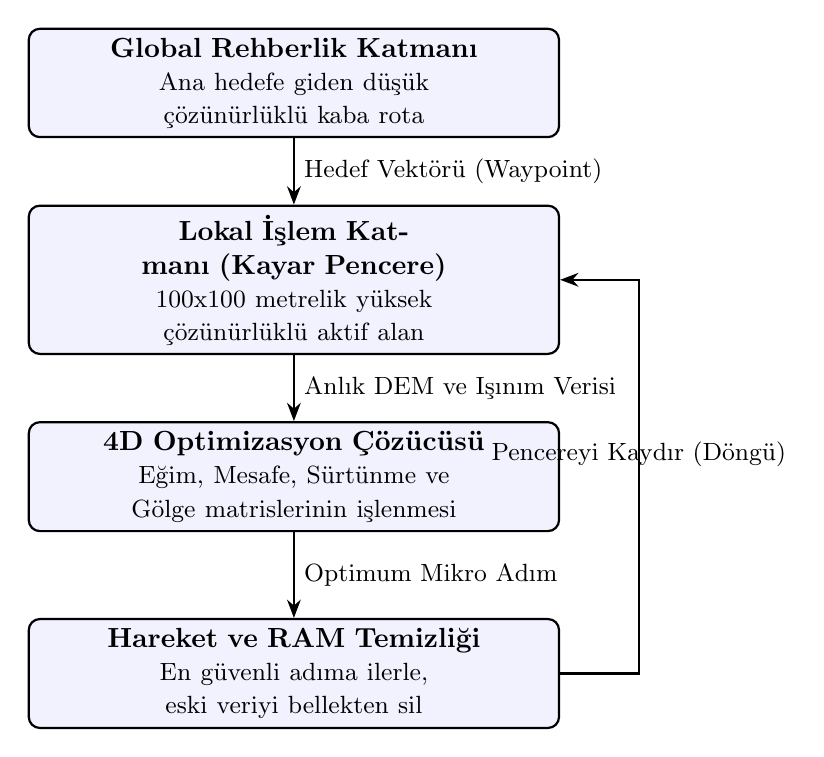
\begin{tikzpicture}[auto,
        box/.style={rectangle, draw=black, fill=blue!5, text width=6.5cm, text centered, rounded corners, minimum height=1.2cm, thick},
        arrow/.style={-{Stealth}, thick}]

        \node (global) [box] at (0, 0) {\textbf{Global Rehberlik Katmanı}\\ \small Ana hedefe giden düşük çözünürlüklü kaba rota};
        \node (local) [box] at (0, -2.5) {\textbf{Lokal İşlem Katmanı (Kayar Pencere)}\\ \small 100x100 metrelik yüksek çözünürlüklü aktif alan};
        \node (cost) [box] at (0, -5.0) {\textbf{4D Optimizasyon Çözücüsü}\\ \small Eğim, Mesafe, Sürtünme ve Gölge matrislerinin işlenmesi};
        \node (move) [box] at (0, -7.5) {\textbf{Hareket ve RAM Temizliği}\\ \small En güvenli adıma ilerle, eski veriyi bellekten sil};

        \draw [arrow] (global) -- node[anchor=west] {\small Hedef Vektörü (Waypoint)} (local);
        \draw [arrow] (local) -- node[anchor=west] {\small Anlık DEM ve Işınım Verisi} (cost);
        \draw [arrow] (cost) -- node[anchor=west] {\small Optimum Mikro Adım} (move);
        \draw [arrow] (move.east) -- ++(1,0) |- node[anchor=south, near start] {\small Pencereyi Kaydır (Döngü)} (local.east);
    \end{tikzpicture}
    \caption{Hiyerarşik Kayar Pencere (Sliding Window) ve Çok Amaçlı Optimizasyon Akış Şeması. Düşük kapasiteli donanımlar (RAD750), sadece ihtiyaç duyulan dar bir alanı RAM'de tutarak kilitlenmeleri önler.}
    \label{fig:akis_semasi}
\end{figure}

\begin{itemize}
    \item \textbf{Dinamik Bellek Optimizasyonu:} Sadece pencere içindeki 1 metrelik yüksek çözünürlüklü topoğrafya ve ışın izleme (ray casting) verisi RAM’e yüklenir. Arkada kalan ve işlevi biten veriler bellekten anında silinir, ilerideki veriler ise araç o bölgeye yaklaştıkça parça parça çekilir.
    \item \textbf{Lokal Optimizasyon:} Bir önceki bölümde detaylandırılan Dört Boyutlu Çok Amaçlı Maliyet Fonksiyonu ($C_{toplam}$), tüm haritada değil, sadece bu dar pencere içerisindeki piksellerde koşturulur. Araç, pencere sınırlarına geldiğinde bir sonraki alt hedef noktasını Global Rehberlik Katmanı’ndan alarak yönünü tayin eder.
\end{itemize}
Bu mimari sayesinde uzay aracı; devasa ve bilinmez bir harita üzerinde kaybolmadan, RAD750 gibi kısıtlı bir uzay işlemcisini kilitlemeden ve önüne çıkan 1 metrelik mikro engellerden (kaya, krater, gölge) otonom bir şekilde sıyrılarak ilerleyebilmektedir.

\section{Sonuç ve Gelecek Çalışmalar}
Bu rapor, TUA AYAP-2 hedefleri doğrultusunda geliştirilen, kısıtlı uzay donanımları üzerinde Ay yüzeyinin fiziksel gerçekliklerini (eğim, gölge, regolit) harmanlayarak otonom rota çizebilen bir mimariyi sunmuştur. Geliştirilen Hiyerarşik ve Çok Amaçlı Rota Optimizasyonu, aracın sadece en kısa yolu değil, en "verimli" ve "güvenli" yolu bulmasını sağlayarak hayatta kalma ihtimalini en üst düzeye çıkarmayı hedeflemektedir.

\end{document}
